\begin{figure}[!htbp]
\centering
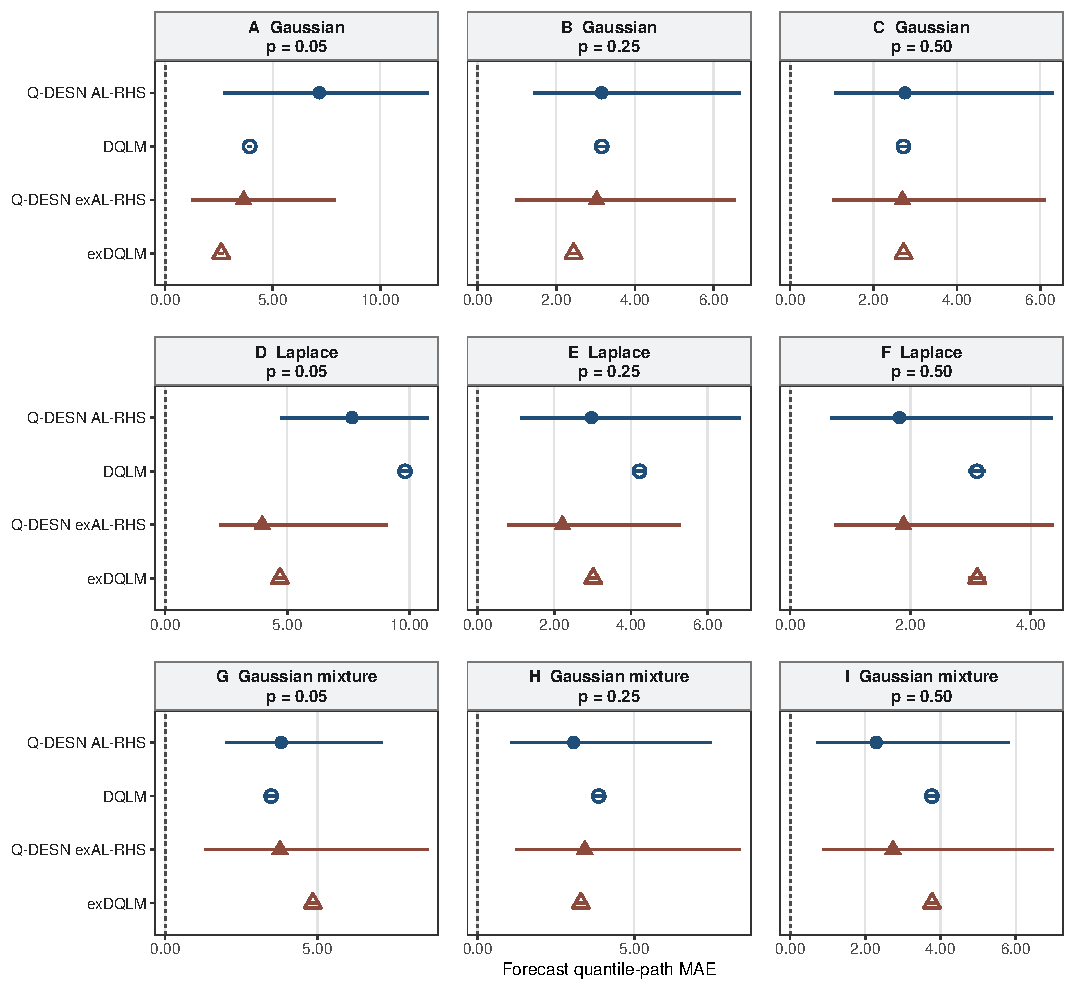
\includegraphics[width=0.98\textwidth]{figures/ch04-qdesn/independent_simulation/qdesn_validation_500obs_v14_mcmc_forecast_mae_intervals.pdf}
\caption{MCMC forecast quantile-path mean absolute error (MAE) in the
single-quantile simulation. Points are posterior means and horizontal segments
are equal-tailed 95\% posterior intervals; lower values are better. Navy
circles identify the \(\AL\) models and muted-brick triangles the \(\exAL\)
models; filled symbols denote Q--DESN and open symbols the corresponding
dynamic quantile linear model. Panels A--I identify the data-generating family
and probability level and use separate horizontal scales. The dashed line
marks the exact data-generating-process value of zero. Intervals condition on
the simulated series, evaluation design, and case-specific selected
specification.}
\figalt{Nine panels compare posterior forecast-MAE means and 95 percent
intervals for four models across three innovation families and three
probability levels. Lower values are better.}
\label{qdesn:fig:simulation-500obs-mcmc-forecast-mae-intervals}
\end{figure}

\begin{figure}[!htbp]
\centering
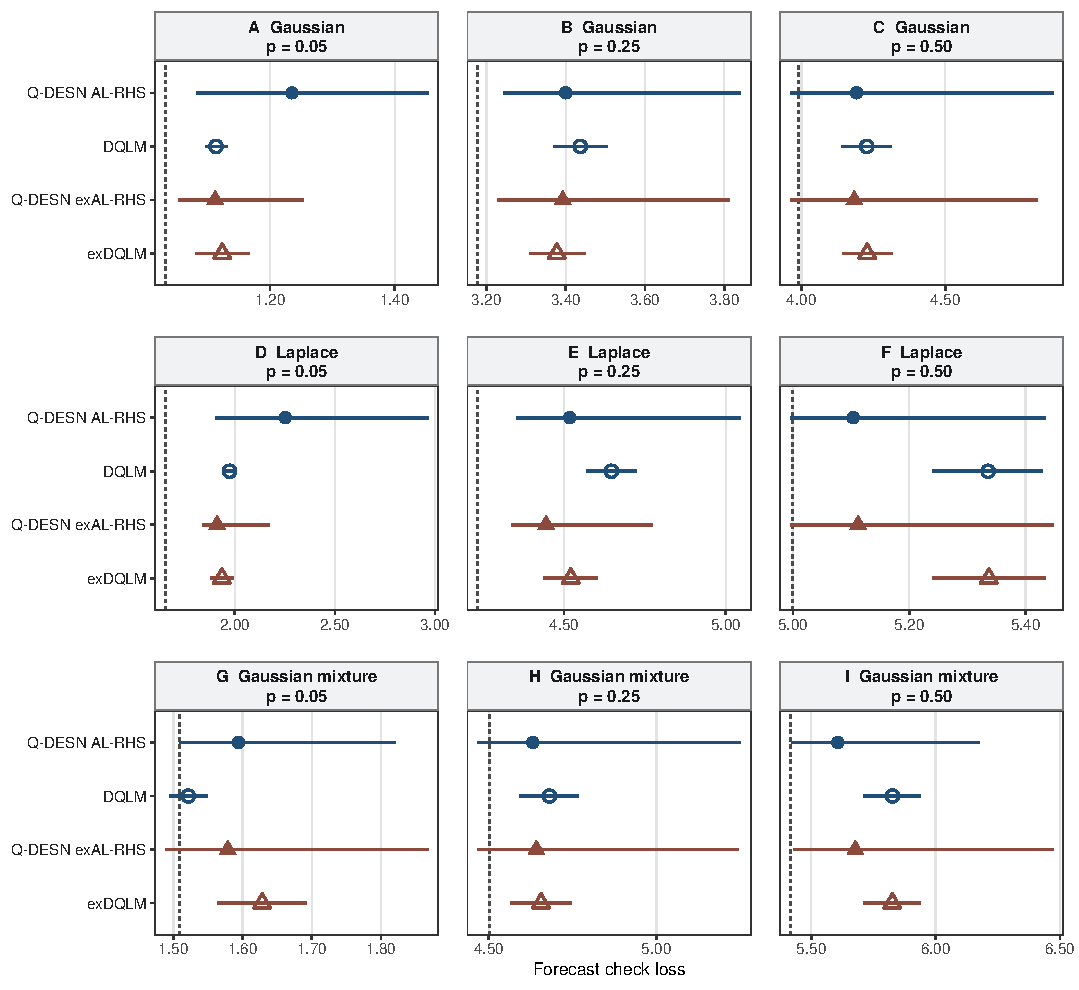
\includegraphics[width=0.98\textwidth]{figures/ch04-qdesn/independent_simulation/qdesn_validation_500obs_v14_mcmc_forecast_check_loss_intervals.pdf}
\caption{MCMC forecast check loss in the single-quantile simulation. Points
are posterior means and horizontal segments are equal-tailed 95\% posterior
intervals; lower values are better. Model encodings and panels are as in
Figure~\ref{qdesn:fig:simulation-500obs-mcmc-forecast-mae-intervals}, with separate
horizontal scales. The dashed line marks population expected check loss at the
true conditional quantile; conditional finite-sample intervals may cross this
reference.}
\figalt{Nine panels compare posterior forecast-check-loss means and 95 percent
intervals for four models across three innovation families and three
probability levels. Lower values are better.}
\label{qdesn:fig:simulation-500obs-mcmc-forecast-check-loss-intervals}
\end{figure}
